\documentclass[french,12pt,a4paper,oneside,notitlepage]{report}
\usepackage[utf8]{inputenc}
\usepackage[T1]{fontenc}
\usepackage{lmodern}
\usepackage[margin=2.5cm]{geometry}
\usepackage[french]{babel}
\usepackage{xcolor}
\usepackage{times}
\usepackage{graphicx}
\usepackage{amsthm}
%\usepackage{fourier}
\usepackage{hyperref}   % links im text
\usepackage{enumerate}  % for advanced numbering of lists
\usepackage{fancyhdr}  
\usepackage{caption}
\usepackage{listings}
%\usepackage{mathtools}
\usepackage{amsmath}   %arraycolsep
\usepackage[protrusion=true,expansion=true]{microtype}
\usepackage{color}
\usepackage{pdflscape}
\makeatletter
\definecolor{bl}{rgb}{0,0.2,0.6}
\let\LaTeX@startsection\@startsection
\renewcommand{\@startsection}[6]{\LaTeX@startsection%
{#1}{#2}{#3}{#4}{#5}{\color{bl}\raggedright #6}}
\renewcommand{\thesection}{\@arabic\c@section}{\color{bl}}
\renewcommand\paragraph{\@startsection{paragraph}{4}{\z@}%
  {-3.25ex\@plus -1ex \@minus -.2ex}%
  {1.5ex \@plus .2ex}%
  {\normalfont\normalsize\bfseries}}
\makeatother

\DeclareCaptionFont{white}{\color{white}}
\DeclareCaptionFormat{listing}{%
  \parbox{\textwidth}{\colorbox{gray}{\parbox{\textwidth}{#1#2#3}}}}
\captionsetup[lstlisting]{format=listing,labelfont=white,textfont=white}
\lstset{frame=lrb,xleftmargin=\fboxsep,xrightmargin=-\fboxsep}

\lstset{
 	language=C++,
% 	captionpos=b,
 	tabsize=3,
 	frame=single,
 	xleftmargin=\fboxsep,
 	xrightmargin=-\fboxsep,
 	keywordstyle=\color{blue},
 	commentstyle=\color{gray},
 	stringstyle=\color{green},
	extendedchars=true,
% 	numbers=left,
 	numberstyle=\tiny,
 	numbersep=5pt,
 	breaklines=true,
 	showstringspaces=false,
 	basicstyle=\footnotesize\ttfamily,
 	emph={label},
 	inputencoding=utf8,
 	extendedchars=true, 	
 	  literate=%
 	  {é}{{\'{e}}}1
 	  {è}{{\`{e}}}1
 	  {ê}{{\^{e}}}1
 	  {ë}{{\¨{e}}}1
 	  {û}{{\^{u}}}1
 	  {ù}{{\`{u}}}1
 	  {â}{{\^{a}}}1
 	  {à}{{\`{a}}}1
 	  {î}{{\^{i}}}1
 	  {ç}{{\c{c}}}1
 	  {Ç}{{\c{C}}}1
 	  {É}{{\'{E}}}1
 	  {Ê}{{\^{E}}}1
 	  {À}{{\`{A}}}1
 	  {Â}{{\^{A}}}1
 	  {Î}{{\^{I}}}1	
}



%Page
% type user-defined commands here
\begin{document}
\title{RAPPORT DU PROJET 3\\
  Études et expérimentation de la classification des scènes naturelles}   % 
  \author{Rédigé par:\\
      Nguyen Van Tho \& Nguyen Quoc Khai\vspace{1cm}\\
  Sous la supervision de :\\
  Mr HO Tuong Vinh}         

%\date{ Décembre, 2013}    % type date between braces

\maketitle

\section{Introduction}
% Demarche qui est fait
% - comment obtenir des descripteurs?
% - la methode pour reconnaitre le document
%  
% Le résultat, expérimentation, expliquer pourquoi avoir ces résultats?
% Perspective: qu'est-ce qui peut fait pour améliorer le travail?
La reconnaissance et la catégorie des images sont importantes pour accéder à l'information visuelle au niveau d'objets et de types de
scènes. Pour l'instant, un des types de reconnaissances le plus difficile est la reconnaissance des scènes naturelles.
En fait, ce type de reconnaissance est défié par les défis tel ques la variation de point 
de vue, la
différence d'échelle, le changement d'illumination, le désordre du fond, l'occlusion
et la déformation. 

La reconnaissance des scènes naturelles ont beaucoup d'application dans plusieurs domaines
notamment la recherche d'images, la reconnaissance de location, ...
\
\section{État de l'art}
Plusieurs techniques ont été proposées au cours de ces dernières années afin de faciliter la classification des scènes naturelles. Les méthodes au dessous permet décrire les idées principales des méthodes étudiées au cours la durée de ce TP.

\pagebreak
\subsection{Approche par mots visuels « Visual Word »}
\subsubsection{Caractéristiques : }
On peut voir l'idée de cette méthode par l'image ci-dessous :
\begin{figure}[ht]
	\begin{center}
	  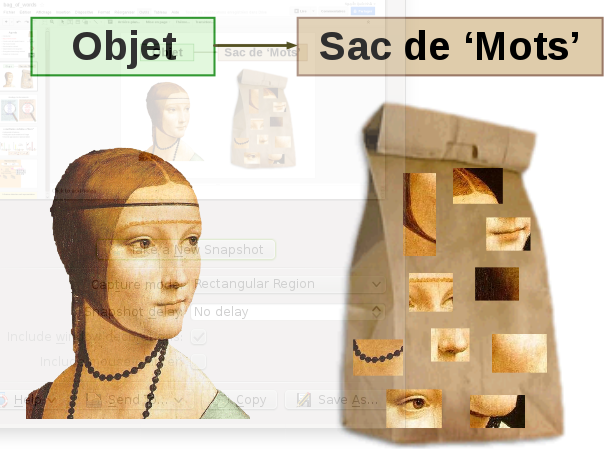
\includegraphics[width=8cm]{img1.png}
	\end{center}
	 \caption{Idée de la méthode « mots visuels »}
\end{figure}\\

Cette méthode obtient des caractéristiques locales de l'image : région « stables », points d'intérêt (SIFT, SURF...), etc. Ensuite, elle trouve des caractéristiques qui se répètent dans les images (construction d'un vocabulaire). Dans cette méthode, une image est décrite par les mots visuels qu'elle contient. Ces mots ne sont pas dans l'ordre. Dans cette méthode, on considère une image comme un sac de mots visuels.

\subsubsection{Algorithme}
On peut décrire la méthode mots visuels en 3 étapes :
\begin{enumerate}
\item Trouver les caractéristiques stables des images
\item Construire un dictionnaire par calculer les histogrammes
\item Décrire chaque image comme un sac de mots visuels
\end{enumerate}

\subsubsection{Reconnaissance par mots visuels}
Après avoir détecté des caractéristiques et construit d'un dictionnaire, cette méthode peut reconnaitre ou classifier des objets en comparant le sac de mots de chaque image de test avec les sacs de mots des images d'apprentissage.\\

\pagebreak
La méthode mots visuels peut être résumé par cette image :
\begin{figure}[ht]
	\begin{center}
	  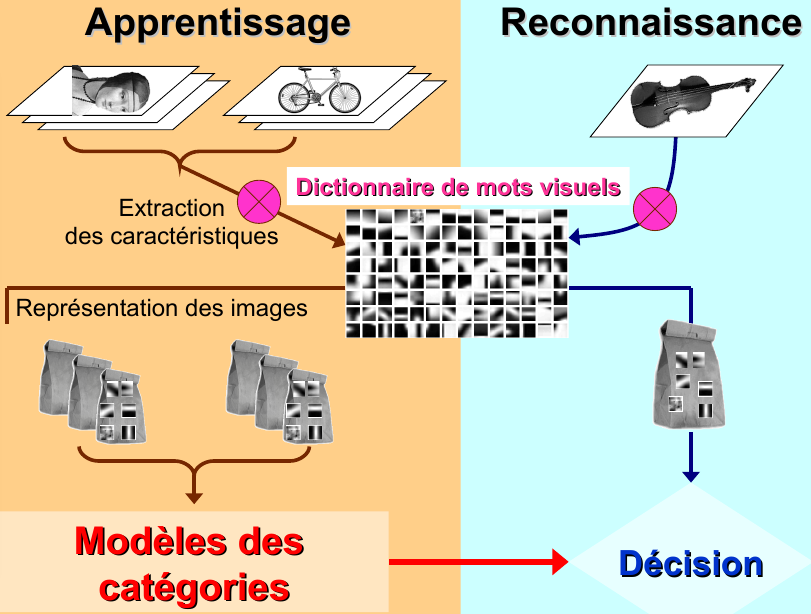
\includegraphics[width=8cm]{img2.png}
	\end{center}
	 \caption{Résumé de la méthode « mots visuels »}
\end{figure}\\

\subsection{Méthode Beyond Bags of Features : Spatial Pyramid Matching}
Basée sur la même idée avec la méthode bag of visual word, cette méthode prend aussi des points intérêts et construit les vocabulaires. Autrement dit, la méthode <<Spatial Pyramid Matching>> est différente dans l'étape de faire la correspondance.

\subsubsection{Pyramid Match Kernels}
Cette méthode divise l'image en des bloques pour faire la correspondance et en des niveaux différents. Dans les niveaux différents, le nombre de bloques divisés est différent. Le nombre de bloques est augmenté quand le niveau augmente. $l$ signifie le niveau. $l = 0, 1, 2, ..., L$.
Une fois que l'on a calculé les histogrammes, le nombre de correspondance est calculé par l'histogramme d'intersection :
\begin{equation}
I(H^l_X,H^l_Y) = \sum_{i=1}^{D} min(H^l_X(i),H^l_Y(i))
\end{equation}
\textit{X, Y sont deux ensembles de points que l'on veut faire la correspondance.}\\
\textit{$H^l_X, H^l_Y$ sont les histogrammes (nombre de points) de X et de Y au niveau $l$.}\\
\textit{$D$ est le nombre de bloques et $H^l_X(i)$ est l'histogramme de $X$ au niveau $l$ dans le bloque $i$}\\
\textit{Pour plus simple, on écrit $I^l$ au lieu de $I(H^l_X,H^l_Y)$}\\

Pour calculer le $I$ au niveau $L$, on applique exactement cette formule, mais pour les autres niveaux $l = 0, 1, ..., L-1$, on recalcule le nouveau $I$ comme ci-dessous : 
\begin{equation}
I^l = I^l - I^{l+1}
\end{equation}

Après avoir calculé tous les $L I$ pour tous les niveaux, on calcule $I$ total comme cette formule :
\begin{equation}
I = \sum_{l=0}^{L} \frac{1}{2^{L - l}} I^l
\end{equation}

On peut voir un exemple de calculer les histogrammes des trois niveaux dans l'image ci-dessous :
\begin{figure}[ht]
	\begin{center}
	  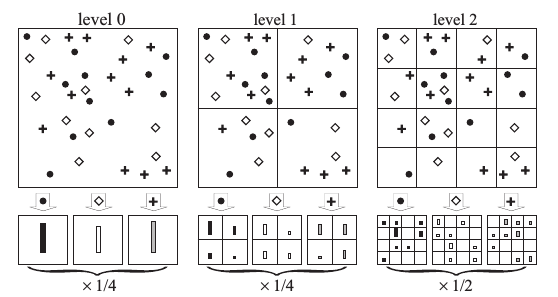
\includegraphics[width=8cm]{img3.png}
	\end{center}
	 \caption{Exemple de trois niveaux de la méthode Pyramid Matching}
\end{figure}

\pagebreak
\section{Méthodes proposées}
En cherchant une méthode qui rend un résultat acceptable et qui est faisable dans le 
carde un projet universitaire, nous avons choisi parmi les méthodes présentées dans la 
partie l'état de l'art la méthode "bag of visual word". En effet, cette méthode est une 
combinaison de plusieurs méthodes. La méthode a des étapes suivantes: 
\begin{itemize}
 \item Détection des points d'intérêt et ses descripteurs
 \item Regroupement (Cluster) ces descripteurs pour définir un dictionnaire des mots, 
chaque centroïde est un mot 
 \item Calcul les histogrammes de mots des images d'apprentissage selon le dictionnaire
 \item Classification les images de test en utilisant les histogrammes de mots
\end{itemize}

À chaque étape, on peut utiliser des méthodes différente. Nous choisissons la méthode 
SIFT afin d'extraire les points d'intérêt et ses descripteurs. En suite, la méthode 
Kmeans [1] est utilisée pour le regroupement des descripteurs afin de définir un 
dictionnaire.
Pour la tâche de classification nous choisissons la méthode support vector machine (SVM) 
[2] qui rend un bon résultat et qui est vérifié dans l'était de l'art. Nous avons 
expérimenté 2 noyaux: linaire et RBF (Gaussien), le résultat de notre expérimentation 
montre que le noyau gaussien est plus approprié au ce genre de problème. Donc, nous 
ne présentons que le résultat avec le noyau gaussien.

\section{Expérimentation}
Nous avons fait plusieurs expérimentation afin d'évaluer notre approche et d'examiner l'impact du nombre de scène et de
nombre des images sur le résultat. D'abord, nous fixons le nombre de mot du vocabulaire 
de 1000 et trouver les valeur optimale des autres paramètres de SVM. En suite, en 
utilisant ces valeurs optimales, nous expérimentons plusieurs valeur de taille du 
vocabulaire.
\subsection{Critères d'évaluation}
 Dans le but d’avoir une vue plus précise des performances de notre programme, nous 
utilisons  
  les indicateurs suivants :
  \begin{itemize}
   \item Matrice de confusion, le taux de rappel et le taux de précision de chaque scène. 
Cela est pour une analyse plus détaille
  \item Taux de reconnaissance (taux) qui est le rapport du nombre de bonnes 
reconnaissances par 
  le nombre total. 
  \item Temps d'apprentissage du programme
  \item Temps de reconnaissance
  \end{itemize}

\subsection{Méthode d'évaluation}
Nous appliquons la méthode d'évaluation k-fold cross validation afin d'assurer que notre 
programme va bien prédire les nouvelles données. Nous choisissons 3 pour 
la valeur de k. Autrement dit, nous divisons les données en trois ensembles et chaque 
expérimentation nous prenons un ensemble  la validation et deux autres ensembles pour 
l'apprentissage. En effet, avant de diviser les données, nous avons les ordonné 
aléatoirement afin de recevoir un résultat plus précis. La figure 4 l'explique notre 
méthode d'évaluation. Le résultat présenté dans ce rapport est la moyenne de 3 fois 
d'expérimentations.

\begin{figure}[ht]
	\begin{center}
	  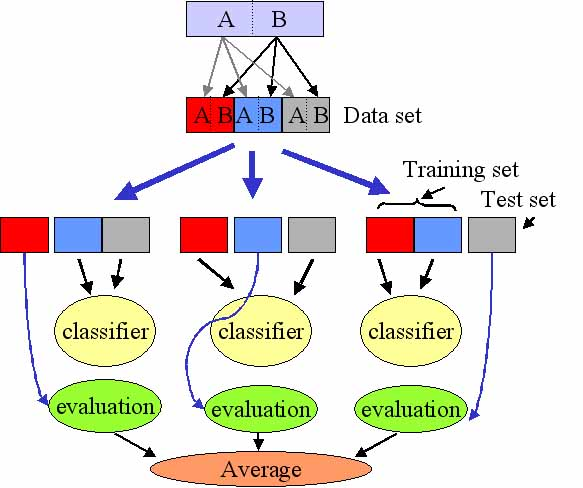
\includegraphics[width=8cm]{3fold.jpg}
	\end{center}
	 \caption{Méthode 3-fold cross validation utilisée}
\end{figure}
\subsection{Scénarios}
\subsubsection{Expérimentation avec une partie des données}
Vu que le temps de calcul de programme est élevé, nous l'expérimentons pour but de 
trouver les valeurs optimales de c et gamma de SVM. De plus, nous souhaitons examiner 
l'impact de nombre de scène en constatant que le taux de reconnaissance diminue quand le 
nombre de scène augmente. Le tableau ci-dessous présente les paramètres que nous 
utilisons pour cette expérimentation. D'abord, nous expérimentons avec la valeur fixée de 
C (300) alors que la valeur de gamma est variée de 0.05 à 2.0. La valeur optimale de 
gamma est ensuite utilisée pour trouver la valeur optimale de C.

\begin{table}[!ht]
  \begin{center}
	\begin{tabular}{|l|l|l|l|}
	  \hline
	  C& gamma & Nombre de scène & Nombre d'image / scène\\
	  \hline
	  300 & 0.05 0.1 0.5 1.0 2.0 & 13 & 120\\
	  \hline
	  10 100 200 300 400 500 & gamma optimale & 13 & 120\\
	  \hline
	\end{tabular}
  \end{center}
\end{table}

\begin{figure}[ht]
	\begin{center}
	  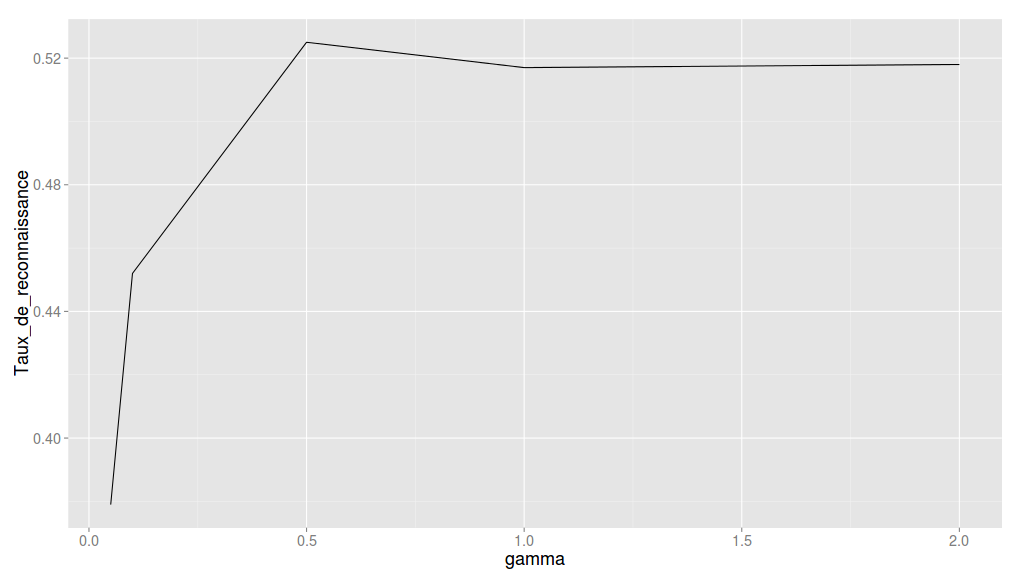
\includegraphics[width=12cm]{findgamma.png}
	\end{center}
	 \caption{Taux de reconnaissance avec une valeur fixée de C = 300 et des variation de 
gamma}
\end{figure}

Au vu des les taux de reconnaissance dans la figure ci-dessus, nous pouvons choisir la 
valeur optimale pour gamma. Avec la une valeur de gamma de 0.5, nous obtenons le taux 
maximum de reconnaissance. Nous allons utiliser cette valeur pour l'étape suivante: 
trouver la valeur optimale de C.

\begin{figure}[ht]
	\begin{center}
	  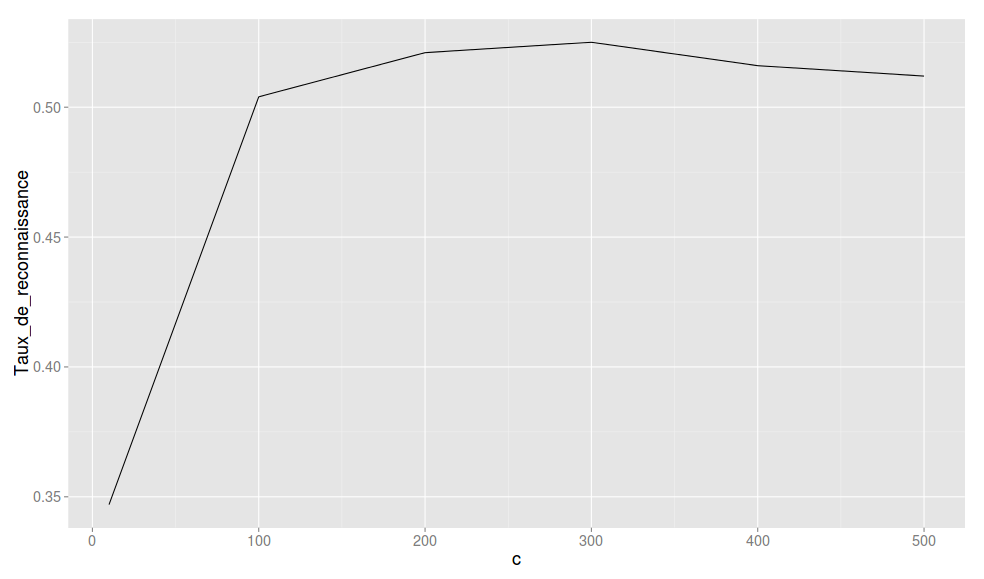
\includegraphics[width=12cm]{findc.png}
	\end{center}
	 \caption{Taux de reconnaissance avec une valeur fixée de gamma = 0.5 et des 
variation de C}
\end{figure}

En voyant la figure ci-dessus nous constatons que la valeur optimale de C est 300. Nous 
allons utiliser cette valeur de C et la valeur de gamma = 0.5 pour les autres 
expérimentations.

\subsubsection{Expérimentation avec les valeurs différentes de la taille de vocabulaire }
La taille de vocabulaire influence beaucoup le taux de reconnaissance [3]. Nous voulons 
donc expérimenter plusieurs valeurs de la taille de vocabulaire afin de trouver la 
meilleure valeur. De plus, nous expérimentons le programme avec toutes les données et 
avec les paramètres optimales.
\pagebreak
\begin{table}[!ht]
  \begin{center}
	\begin{tabular}{|l|l|l|l|l|}
	  \hline
	  Taille de vocabulaire& C& gamma & Nombre de scène & Nombre d'image / scène\\
	  \hline
	  500, 1000, 2000, 5000 & 300 & 0.5 & 13 & maximum\\
	  \hline
	\end{tabular}
  \end{center}
\end{table}

\begin{figure}[ht]
	\begin{center}
	  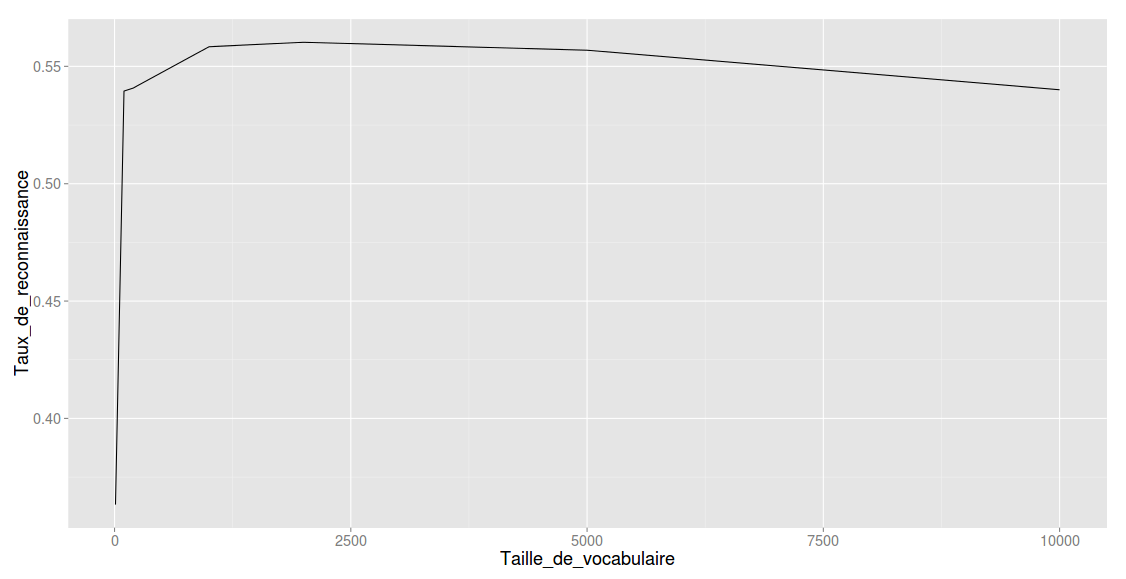
\includegraphics[width=10cm]{dictionarySize.png}
	\end{center}
	 \caption{Taux de reconnaissance avec des tailles différentes du vocabulaire}
\end{figure}
\begin{figure}[ht]
	\begin{center}
	  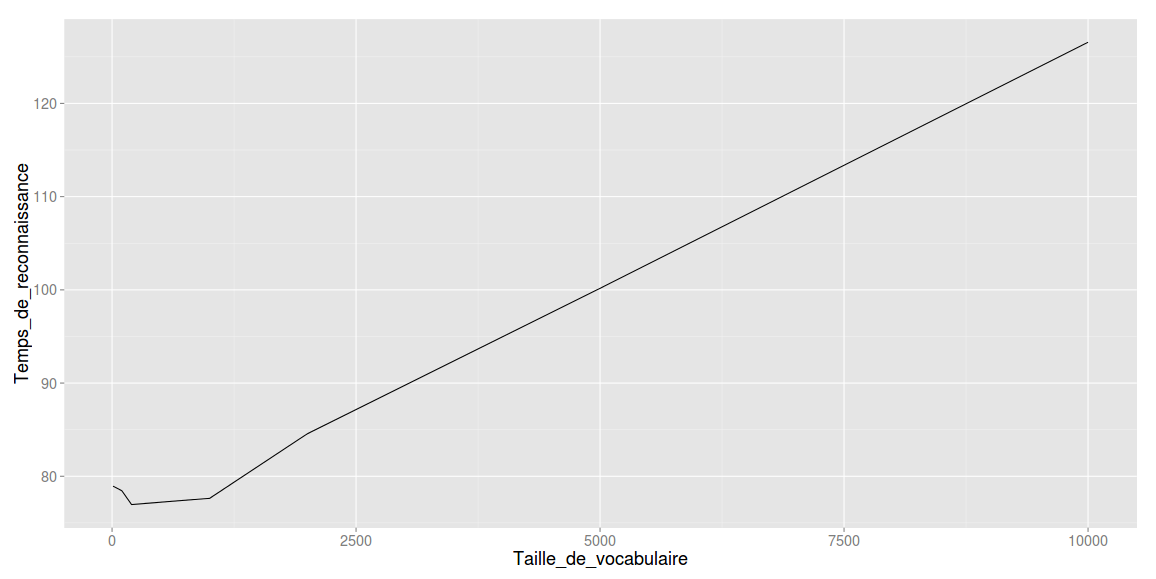
\includegraphics[width=10cm]{time.png}
	\end{center}
	 \caption{Temps de reconnaissance avec des tailles différentes du vocabulaire}
\end{figure}
\begin{figure}[ht]
	\begin{center}
	  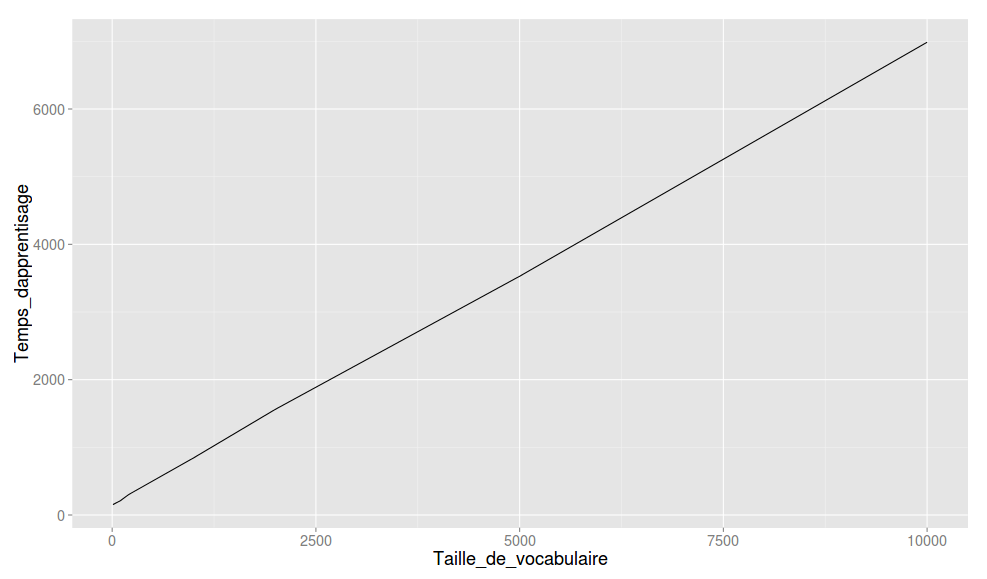
\includegraphics[width=10cm]{ta.png}
	\end{center}
	 \caption{Temps d'aprentissage avec des tailles différentes du vocabulaire}
\end{figure}
\begin{table}[!ht]
	\begin{center}
	\resizebox{\textwidth}{!}{%
	    \begin{tabular}{|l|l|l|l|l|l|l|l|l|l|l|l|l|l|l|}
		  \hline
		 &1&2&3&4&5&6&7&8&9&10&11&12&13&Taux de rappel(\%)\\
\hline
1&69&0&1&0&0&1&1&0&2&1&0&0&6&85.2\\
\hline
2&8&47&5&13&2&9&20&4&2&5&2&0&3&39.2\\
\hline
3&2&0&103&0&0&4&1&0&0&0&0&0&0&93.6\\
\hline
4&4&4&0&35&10&3&7&13&5&1&0&1&5&39.8\\
\hline
5&0&1&1&0&64&0&0&24&8&0&0&2&4&61.5\\
\hline
6&7&1&19&1&0&77&17&4&0&0&0&0&0&61.1\\
\hline
7&1&10&42&3&1&17&57&5&1&0&0&0&1&41.3\\
\hline
8&1&0&1&0&10&5&3&64&11&0&0&0&3&65.3\\
\hline
9&10&0&5&0&4&8&1&14&63&4&0&1&10&52.5\\
\hline
10&2&0&0&0&5&0&0&0&4&36&0&1&25&49.3\\
\hline
11&3&0&0&0&5&2&2&7&4&7&7&4&31&9.7\\
\hline
12&1&0&0&0&7&0&0&5&3&4&3&12&35&17.1\\
\hline
13&7&0&0&0&6&3&0&3&10&5&0&1&62&63.9\\
\hline
p(\%) &60.0&74.6&58.2&67.3&56.1&59.7&52.3&44.8&55.8&57.1&58.3&54.5&33.5&\\
\hline
	    \end{tabular}
}
	    \caption{La matrice de confusion avec la taille de vocabulaire 10000}
	\end{center}
\end{table}
\pagebreak
À partir du résultat de cette expérimentation nous pouvons conclure que la taille du 
vocabulaire influence le taux de reconnaissance. En fait, dans notre cas, la 
taille de vocabulaire optimale est environ 2000. Le taux de reconnaissance plus grand 
obtenue est 56\% avec la taille de vocabulaire de 2000 et les paramètres de SVM c=300 et 
gamma = 0.5.
En voyant la figure 9, on constate que le temps d'apprentissage augmente linéairement 
quand la taille de vocabulaire augmente. Quand cette taille égale 10, le temps 
d'apprentissage est 154 seconds, quand la taille égale 10000, le temps est 6986 seconds. 
Cependant, le temps de reconnaissance augmente très lentement par rapport à 
l'augmentation de la taille de vocabulaire (figure 8). Par exemple, quand la taille de 
vocabulaire est 10, le temps de reconnaissance (une reconnaissance de 1290 images) est 79 
seconds et celui quand la taille est 10000 est seulement 126 seconds.
On peut conclure que quand la taille de vocabulaire augmente, le temps pour 
l'apprentissage augmente beaucoup mais le temps pour la reconnaissance augmente un peu.

\subsubsection{Analyses sur la matrice de confusion}
Au vu la matrice de confusion (Table 1) on constate qu'il y a deux scènes que le 
programme ne reconnaît pas bien, ce sont la scène 11 et 12 (bedroom et kitchen), les taux
de rappels sont 9.7 et 17.1\%. Elles sont mal classifiées à la scène 13 (living room). On 
peut expliquer que dans ces images, il y a beaucoup d'objets ressembles tels que: table, 
chaise, lampe ...

Nous allons faire une autre expérimentation sans les scènes à intérieurs (sans scène 11, 
12, 13). Le résultat de cette expérimentation est meilleur avec le taux de reconnaissance 
de 66\%. Le tableau 2 est la matrice de confusion de cette expérimentation. Ce résultat 
montre que notre algorithme rend de meilleurs résultats sur les scènes à l'extérieurs, 
les résultats des scènes à l'intérieur sont moins bons.

\begin{table}[!ht]
	\begin{center}
	    \begin{tabular}{|l|l|l|l|l|l|l|l|l|l|l|l|}
		  \hline
		 &1&2&3&4&5&6&7&8&9&10&Taux de rappel\\
\hline
		1&76&0&0&0&0&0&2&0&1&1&95.0\\
\hline
2&7&65&2&18&1&9&12&2&0&4&54.2\\
\hline
3&1&0&95&0&0&4&9&0&0&0&87.2\\
\hline
4&6&13&1&39&10&1&5&6&3&2&45.3\\
\hline
5&1&0&1&0&71&0&1&15&9&4&69.6\\
\hline
6&5&4&8&1&0&81&22&2&0&1&65.3\\
\hline
7&7&9&32&2&1&19&63&2&1&0&46.3\\
\hline
8&1&1&1&0&13&3&8&60&10&0&61.9\\
\hline
9&11&0&2&0&9&2&4&16&70&4&59.3\\
\hline
10&1&0&0&0&2&0&0&1&1&66&93.0\\
\hline
p&65.5&70.7&66.9&65.0&66.4&68.1&50.0&57.7&73.7&80.5&\\ 
\hline
	    \end{tabular}
	    \caption{La matrice de confusion avec la taille de vocabulaire 1000, sans les 
scènes: living room, bedroom, kitchen}
	\end{center}
\end{table}
\pagebreak
\section{Conclusion}
Dans ce domaine, il y a des méthodes qui permettent de classifier bien deux catégories mais pour plusieurs catégories, elles ne classifient pas bien, pour cela on perd de temps pour essayer.\\
Durant ce TP, on a faire la recherche sur le domaine de classification des scènes 
naturelles, cherche à comprendre quelques méthodes tels que Pyramid Match Kernels, Bag of 
Visual Words, etc. Finalement, on a implémenté la méthode Bag of Visual Words. Bien qu'il 
y a des défis dans ce domaine, on ait réussi à implémenter une méthode qui sert à 
classifier les catégories d'images avec le résultat acceptable.\\
Nous avons expérimenté plusieurs scénarios. Le résultat de notre programme montre que la 
reconnaissance des scènes à l'intérieur est plus difficile que celle des scènes à 
l'extérieur. 
\begin{thebibliography}{9}
\bibitem{r1}
  Jun Hartigan, John A., and Manchek A. Wong.
  \emph{Algorithm AS 136: A k-means clustering algorithm.}.
  Journal of the Royal Statistical Society. Series C (Applied Statistics) 28.1 (1979): 100-108.
  
\bibitem{r2}
  Burges, Christopher JC
  \emph{A tutorial on support vector machines for pattern recognition.}.
  Data mining and knowledge discovery 2.2 (1998): 121-167. APA	
  
\bibitem{r3}
	Yang, Jun, et al.
  \emph{Evaluating bag-of-visual-words representations in scene classification.}.
  Proceedings of the international workshop on Workshop on multimedia information retrieval. ACM, 2007.

\bibitem{c1}
  Jun Yang, Yu-Gang Jiang, Alexander G. Hauptmann, Chong-Wah Ngo
  \emph{EvaluatingBag-of-Visual-Words RepresentationsClassification}.

\bibitem{c2}
  Svetlana Lazebnik, Cordelia Schmid, Jean Ponce.
  \emph{Beyond Bags of Features: Spatial Pyramid Matching for Recognizing Natural Scene Categories}
  
\bibitem{c3}
  NGUYEN Thi Oanh 2013,
  \emph{transparent sur Bag of Visual Words, IFI Hanoi}.
  
\end{thebibliography}

\end{document}
